\section{Verwandte Arbeiten}

In der Literatur gibt es mehrere Artikel, die Ansätze
zur Automatisierung des Testens von Webanwendungen
vorstellen (vgl. \cite{6140672} und \cite{6211171}).
Die meisten dieser Ansätze folgen den Schritten zum
Schreiben von UI-Tests, die in \autoref{sec:verschiedene-schritte-zur-erstellung-einer-testsuite}
beschrieben  wurde. Für die Erstellung eines Test Automation
Framework mit Selenium wählten Fei Wang et al.
(vgl. \cite{6211171}) zunächst die verschiedenen
Webbrowser aus, die sie für die Entwicklung der
Tests verwenden wollten. Anschließend erstellten
sie eine Testumgebung. Diese Umgebung sollte mit
generierten Testdaten erstellt werden. Dann folgt
die Phase des Designs von Testfällen, die sie in
ein Set von Aktionen übersetzen werden. Diese Aktionen
werden dann in verschiedene Befehle/Skripte übersetzt,
je nach dem, welches Tool zum Testen verwendet wird
(in diesem Fall Selenium). Danach werden die Aktionen
von dem verwendeten Testwerkzeug ausgeführt und
ein Testbericht erstellt.


Die letzte Phase besteht aus dem Testen des
Test-Frameworks und seiner Infrastruktur. Die
Leistung in Bezug auf Wiederverwendbarkeit,
Erweiterbarkeit und Kompatibilität muss bewertet werden.
Um diese Tests durchzuführen, empfehlen Fei Wang
et al. die Verwendung unterschiedlicher Testdaten bei
der Vorbereitung der Testfelder und die Beobachtung der
erzielten Ergebnisse. Die Ergebnisse der Evaluierung
des webbasierten Testautomatisierungs-Frameworks haben
gezeigt, dass das Framework den Testern ein Werkzeug
gibt, mit dem sie bequem verschiedene Browser für den
Test von Webanwendungen konfigurieren, eine große
Menge an Daten für den Leistungstest vorbereiten
können, indem sie die Datenressourcen direkt
konfigurieren, einen Testtyp einfach konfigurieren,
indem sie einen Testtyp modifizieren, und zwischen
verschiedenen Tests umschalten können, ohne
irgendwelche Elemente im Zusammenhang mit den
Testfällen zu verändern (vgl. \cite{6211171}).

\begin{figure}[H]
    \centering
    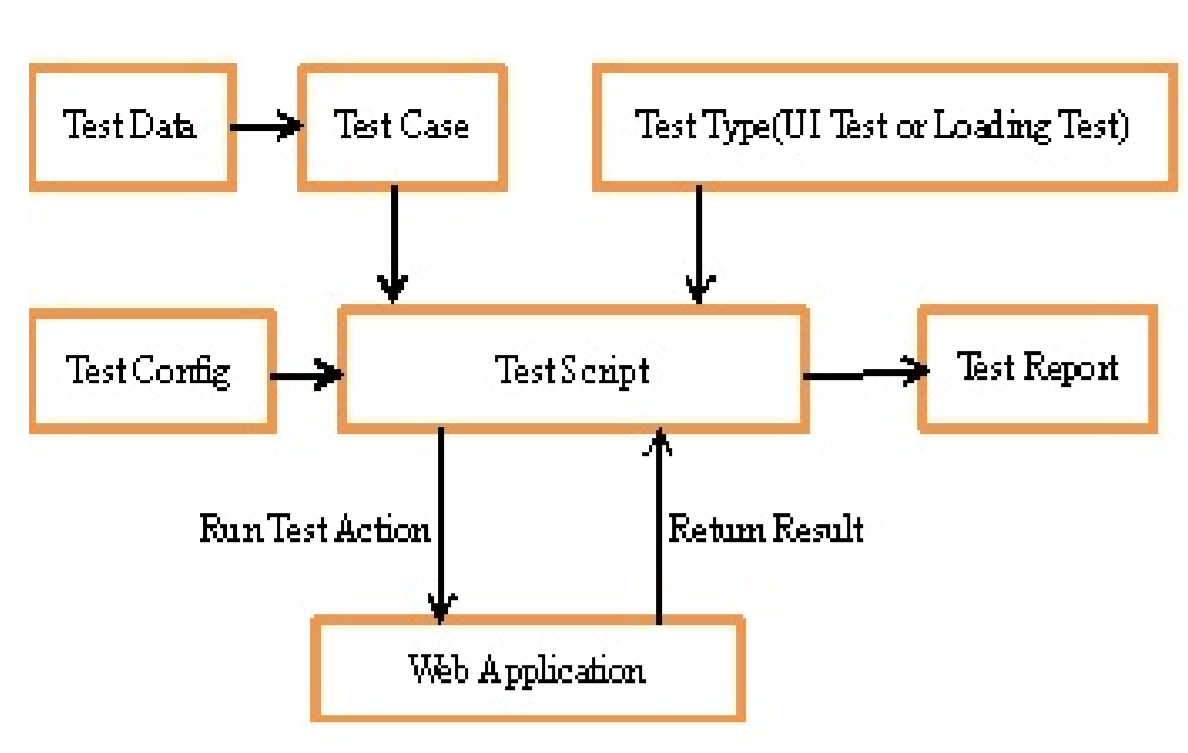
\includegraphics[scale=0.5]{images/web-based}
    \caption{Funktionsweise eines WebAutomationTesting-Frameworks (vgl. \cite{6211171})} \label{fig:web-based}
\end{figure}


